\chapter{Trabalho Proposto} \label{cap:tp}
%2345678901234567890123456789012345678901234567890123456789012345678901234567890

\todo{rever no final do cap}
O trabalho visa dois objetivos principais: (i) apoiar o desenvolvimento de
aplicações; (ii) minimizar a dificuldade de configuração existente. O primeiro
objetivo é alcançado com a construção de artefatos de software que leem e
questionam as ontologias via Jason. O segundo objetivo é alcançado pela
criação das ontologias que, além de fazerem o raciocínio, definem um
vocabulário básico a ser conhecido. Por exemplo, um desenvolvedor só
precisa conhecer a ontologia de ambiente proposta para saber\dev{} o que o agente
deve enviar de crenças ou percepções e o que esperar em retorno.

Esse capítulo visa mostrar de maneira organizada a ideia proposta e
desenvolvida. Dessa forma, a primeira seção apresenta a ideia geral do
trabalho sendo proposto. A seguir, a ontologia do modelo afetivo é
apresentada. Em seguida, a ontologia do modelo de percepções é mostrado. Por
fim, a ontologia do modelo de humanos virtuais é discutida e como foi feito a
junção com a mesma.
% cuidar com as palavras: seção, ontologia, modelo

\section{Ontologia Afetiva} \label{cap:tp:oa}

A fundamentação do modelo afetivo sendo utilizado aqui é o proposto por
\citet{ortony1988cse} e encontra-se explicado na seção \ref{cap:eda:mce}
\todo{talvez trocar por uma mais especifica?}. A ontologia proposta tinha
como ideia inicial não utilizar regras, porém como pode ser observado na
Tabela~\ref{tab:oa:geral} foi necessário a criação de regras para suportar o
raciocínio no nível de indivíduo. As regras que ajudam a conclusão das
relações \emph{hasKnow}, \emph{hasFriend} e \emph{hasEnemy} são diferentes das
demais por causa que elas tem como característica operar no domínio e na
imagem da classe \emph{Agent}. Por exemplo\todo{fazer?}, se Fulano
avalia que se relaciona bem com o Ciclano então Fulano tem amigo Ciclano. Note
que o contrario não é necessariamente verdade, o Ciclano pode apenas saber que
conhece o Fulano.

\begin{table}
	\caption{Ontologia proposta com expressividade: ALCHIN(D).}
	\label{tab:oa:geral}
	\begin{center}
	\begin{tabular}{|c|c|}
	%\begin{tabular}{|p{34mm}|p{50mm}|p{50mm}|}
		\hline
		Descrição & Quantidade \\ \hline
		Classes &  45 		\\ \hline
		Propriedade de Objetos & 16 \\ \hline
		Propriedade de Dados & 14 \\ \hline
		Indivíduos &  0		\\ \hline
		Regras & 7 \\ \hline
	\end{tabular}
	\end{center}
\end{table}

Na Figura~\ref{fig:rlocc}, as regras utilizaram funções para verificar se
um indivíduo é diferente do outro. Assim, recomenda-se fortemente que quando
se registrar um indivíduo da classe \emph{Object} ou \emph{Agent} que a
informação de igualdade ou diferenciação seja preenchida\dev{}. Assim, se
evita que o raciocinador conclua que não conhece a resposta.

\begin{figure}[t]
  \centering
  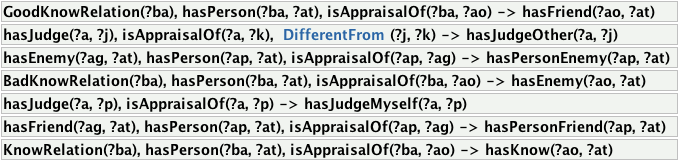
\includegraphics[width=14cm]{figuras/rules-LOCC.png}
  \caption{Regras da ontologia proposta.}
  \label{fig:rlocc}
\end{figure}

A Figura~\ref{fig:kplocc} mostra a árvore de relações que tem como imagem
dados ou instâncias (objetos). Ao olhar se comparar as Figuras~\ref{fig:rlocc}
e Figura~\ref{fig:kplocc} se chega a conclusão que as propriedades que as
regras concluem não precisam ser configuradas pelo usuário. Assim, ao invés de
14 propriedades de objetos conforme informado na Tabela~\ref{tab:oa:geral}
apenas 7 precisam ser conhecidas. Dessas a propriedade mais utilizada é a
\emph{hasSomething} que serve para indicar o que esta sendo avaliado. Note que
\emph{hasPerson} deve ser usado quando o indivíduo em avaliação for um membro
da classe \emph{Agent}. Já, a relação \emph{hasJudge} serve para indicar que o
membro da classe \emph{Object} esta sendo avaliado. Por exemplo, uma avaliação
é de Alberto julgando o seu carro em determinada valoração
negativa\todo{fazer?}.

\begin{figure}[b]
  \centering
  \begin{tabular}{cc}
  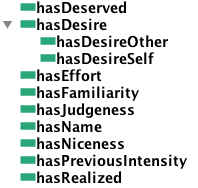
\includegraphics[height=4cm]{figuras/dataProperty-LOCC.png} & 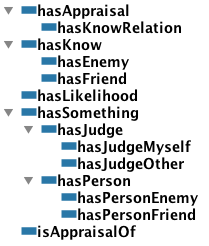
\includegraphics[height=5cm]{figuras/objectProperty-LOCC.png} \\
  (i) Relações de dados & (ii) Relações de Objetos
  \end{tabular}
  \caption{As relações existentes na ontologia proposta.}
  \label{fig:kplocc}
\end{figure}

Todos os dados numéricos da ontologia são inteiros. Isso foi feito com a
finalidade de permitir o usuário normalize\dev{} o número obtido da
maneira que desejar. Além disso, foi tomada a decisão de não especificar o
domínio da maioria das propriedades por causa que isso forçaria um
enquadramento em classes não desejadas. Por exemplo\todo{fazer?}, um indivíduo
com somente a relação \emph{hasLikelihood} seria enquadrado no conceito
\emph{ConsequenceForSelf}, enquanto o correto seria não ser concluído nada,
isto é, pertencer à classe \emph{Thing}.

A estrutura da ontologia pode ser visualizada na Figura~\ref{fig:tlocc}. Além
disso, pode ser recomendável olhar a
Figura~\ref{fig:occ_model}~(pg.~\pageref{fig:occ_model}) do modelo criado por
\citet{ortony1988cse} durante o resto da discussão dessa seção. Os
sub-conceitos de \emph{Emotion} correspondem aos ramos do modelo original.
O ramo \emph{ActionsOfAgents} julga a responsabilidade e o quanto o agente que
realizou uma ação ou evento se desviou do esperado, o de
\emph{ConsequencesOfEvents} julga a consequência de um evento e
\emph{AspectsOfObjects} julga a atração para com um objeto.

O primeiro a ser abordado é, o menos cognitivo, \emph{AspectsOfObjects}.
As emoções desse tipo são relacionadas com atratividade e familiaridade.
Entretanto, essas duas relações foram consideradas equivalentes porque o
importante, para o modelo, é quando ambas são positivas ou ambas são
negativas. Assim sendo, uma pode assumir os dois papeis sem maiores
penalidades e simplificando a modelagem. A emoção \emph{Hate} é modelada como
tendo a propriedade de familiaridade (\emph{hasFamiliarity}) com valores
negativos, enquanto a emoção \emph{Love} tem valoração dessa mesma propriedade
positiva. Caso o valor seja zero, nada pode ser concluído.

\begin{wrapfigure}{r}{0.4\textwidth}
  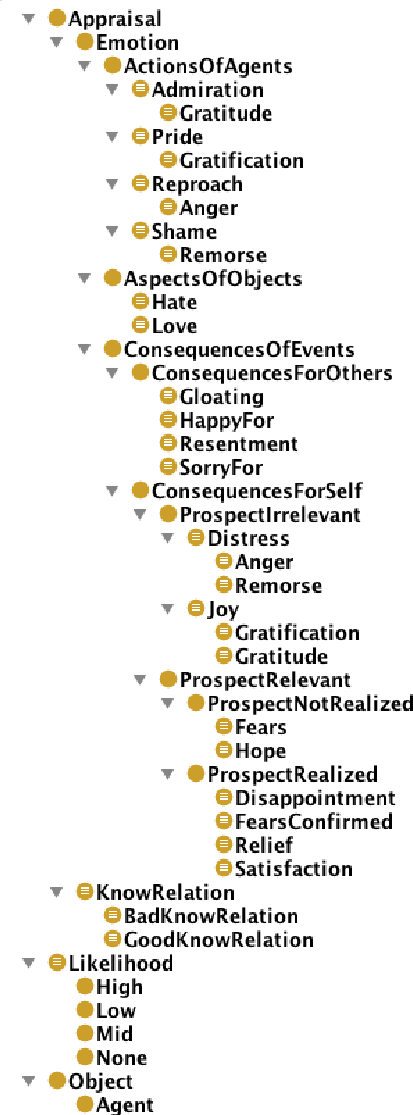
\includegraphics[height=16cm]{figuras/hierarquiaLOCC.png}
  \caption{Taxonomia da ontologia proposta baseado no modelo.}
  \label{fig:tlocc}
\end{wrapfigure}

Cabe notar que parece estranho uma emoção \emph{Love} com um objeto, porém
essa emoção foi escolhida por quem montou o modelo por ser a emoção mais forte
de seu tipo. Assim, níveis menores implicam em outros tipos de emoção. Além
disso, conforme explicado no trabalho, agentes podem ser vistos como objetos
quando se esta avaliando a sua atração. Assim, todo agente (\emph{Agent}) é um
objeto (\emph{Object}). Por exemplo\todo{fazer?}, Alberto odeia Blueriver ou
Millie gosta de rosas vermelhas.

O segundo ramo é chamado \emph{Actions of Agents}, ele pode ser pensado como
um ramo que julga a responsabilidade por uma determinada ação ou evento.
Assim, esse ramo é capaz de gerar 4 emoções: Admiração (\emph{Admiration}),
Orgulho (\emph{Pride}), Vergonha (\emph{Shame}) e Reprovação
(\emph{Reproach}). Por exemplo\todo{fazer?}, Millie possui orgulho por cozinhar ou Jane
reprova seu carro novo (que esta apresentando problemas regularmente).

Na definição, as emoções de orgulho e vergonha podem acontecer mesmo quando se
esta avaliando ações de outras pessoas. Por exemplo, Dolares tem vergonha de
sua mãe (que não cozinha). Essa conclusão é possível por causa de uma relação
que ele propõem chamada força de unidade cognitiva \footnote{Traduzido
literalmente de \emph{Strength of cognitive unit}.}. Como em nenhum momento da
definição, ele dá mais detalhes dessa unidade cognitiva resolveu-se considerar
que vergonha e orgulho são emoções sentidas somente quando o agente esta
avaliando a si mesmo e, dessa forma, o exemplo anterior não é possível.

As emoções que julgam responsabilidade são definidas como tendo uma relação de
julgamento (\emph{hasJudge}) e uma relação que mapeia o valor do julgamento
(\emph{hasJudgeness}) que representa o quanto o agente se desviou do
comportamento esperado, isto é, em casos de aprovação é um valor positivo e em
casos de reprovação é um valor negativo. Todavia, isso ainda não permite
diferenciar a emoção de admiração da emoção de orgulho ou a reprovação da
vergonha. Essa distinção é possível ao se dividir a relação de julgamento com
duas sub-relações: tem auto-julgamento (\emph{hasJudgeMyself}) e tem
julgamento de outro (\emph{hasJudgeOther}).

A utilização de sub-propriedade torna possível escrever a ontologia da maneira
esperada suprindo o problema. Entretanto, para o usuário pode se tornar
complicado ter que lembrar quando utilizar uma sub-propriedade ou outra.
Assim, foi resolvido deixar o usuário sempre utilizar a relação de julgamento
(\emph{hasJudge}) e via 2 regras inferir se é um auto-julgamento ou o
julgamento de outra pessoa. Para essas regras funcionarem da maneira correta,
o usuário deve declarar que os agentes ou objetos são diferentes. Caso isso
não ocorra, o sistema considera que não há informação para verificar se um
individuo é igual ou diferente que o outro e concluir que não conhece a
resposta. Além disso, a relação de julgamento tem como imagem o conceito
\emph{Object}. Dessa forma, os exemplos anteriores são todos válidos.

Cabe salientar que toda avaliação tem pelo menos duas relações. A primeira
relação serve para conhecer quem esta avaliando (\emph{isAppraisalOf}) e a
outra serve para indicar quem ou o que esta sendo avaliado
(\emph{hasSomething}). Em muitas avaliações essa última pode não ser
informada sem nenhum prejuízo. O último, chamado de \emph{Consequences of
Events} é
dividido em: \emph{Consequences for Self}; \emph{Consequences for Others}.
Toda essa divisão foca na consequência de um evento ou ação feito por um
determinado agente. Por exemplo\todo{fazer?}, Millie tem pena de Alberto ou
Alberto tem esperança (de alcançar seu objetivo) ou Blueriver tem satisfação
(por conseguir escapar).

A \emph{Consequences for Others} expressa 4 emoções: \emph{HappyFor},
\emph{SorryFor}, \emph{Gloating} e \emph{Resentment}. Na definição, essas
emoções dependem: do grau de desejabilidade nosso para com o outro; do grau de
desejabilidade que se presume que o outro tenha; do grau de merecimento do
evento; do tipo de relacionamento com a pessoa. Na ontologia proposta, a principal
diferença com o modelo original é que foi considerado que o grau de
desejabilidade nosso para com o outro e o grau de merecimento do evento são os
mesmos. Dessa forma, se pode utilizar apenas três relações para descrever as
4 emoções.

A relação de merecimento (\emph{hasDeserved}) e relação de desejabilidade
presumida (\emph{hasDesireOther}) são avaliadas de acordo com sua valoração
positiva ou negativa. A terceira relação é a que liga o outro individuo/agente
(\emph{hasPerson}) sendo avaliado. Para se ter o conhecimento de quem esta
julgando é uma pessoa amiga (\emph{GoodKnowRelation}) ou inimiga
(\emph{BadKnowRelation}), esses conceitos foram criados e precisam ser
configurados para cada um dos agentes em questão. O agente pode declarar que
só conhece uma pessoa, que conhece e é um amigo ou que conhece e não gosta
dela (inimiga). Entretanto, quem precisa dessa informação é o conceito de
avaliação quando as relações \emph{hasPersonEnemy} e \emph{hasPersonFriend}
precisam ser descobertas.

A \emph{Consequences for Self} é divida ainda entre consequências de eventos
com probabilidade relevante (\emph{ProspectRelevant}) e irrelevante
(\emph{ProspectIrrelevant}). Cabe salientar que esses dois conceitos se
relacionam com probabilidade (\emph{hasLikelihood}), entretanto enquanto o
primeiro conceito se relaciona com a parte não nula. A outra se relaciona
somente com essa. Dessa forma, ambos os conceitos são disjuntos. A classe de
probabilidade relevante pode ser dividida ainda entre possibilidade não
realizada (\emph{ProspectNotRealized}) e realizada (\emph{ProspectRealized}).

As emoções \emph{Hope} e \emph{Fear} fazem parte do conceito
\emph{ProspectNotRealized}. Esse conceito usa as relações \emph{hasLikelihood}
e \emph{hasDesireSelf}. Essa última propriedade é um número que
representa o desejo de se obter ou repudir o evento. Além disso, quando o
evento ocorre a emoção atual pode virar uma emoção do conceito
\emph{ProspectRealized}, isto é, \emph{Fear} pode virar ou
\emph{FearsConfirmed} ou \emph{Relief} e \emph{Hope} pode virar ou
\emph{Disappointment} ou \emph{Satisfaction}.

Esse conceito \emph{ProspectRealized} não se relaciona em nenhum momento com a
relação \emph{hasLikelihood} porque o evento já aconteceu. Ela possui três
relações distintas das anteriores, a primeira é o grau de realização de um evento
(\emph{hasRealized}), isto é, a visão do agente sobre como a consequência do
evento aconteceu. A segunda relação \emph{hasPreviousIntensity} recebe a
valoração da emoção de medo ou esperança do evento que tinha probabilidade e
serve para saber se o evento é um evento bom (esperança) ou ruim (medo). Já, a
terceira \emph{hasEffort} tenta estimar o grau de esforço que foi dispendido
para a atração ou repulsa da consequência do evento.

O conceito \emph{ProspectIrrelevant} é parecido com o conceito
\emph{ProspectRelevant} com a diferença que a relação \emph{hasLikelihood} vai
somente para valores nulos. Alem disso, as emoções desse conceito e do
\emph{ActionsOfAgents} podem ser misturados formando uma composição. A
composição é quando uma emoção pode ser encaixada em mais de uma emoção como
no caso de se estar alegre (\emph{Joy}), orgulhoso (\emph{Pride}) e
gratificado (\emph{Gratification}). Por fim, o conceito \emph{Setup}
\todo{na diss, vale a pena abrir um paragrafo para falar mais do setup} é o
utilizado para manter junto da ontologia criada o limite mínimo para uma
emoção virar sentimento\dev{}.

%a transferencia eh feita pelo sistema;
%os dados sao carregados para memoria e eliminados;
%conforme reparado nao ha decaimento da emocao, a mesma eh instantanea;
%2345678901234567890123456789012345678901234567890123456789012345678901234567890

\section{Reutilizando uma ontologia de Humanos Virtuais} \label{cap:tp:ruodhv}

...

\section{Ontologias de Percepções} \label{cap:tp:odp}
% de percepcoes virou do ambiente
% voltou a ser de percepcoes

... Última coisa

Uma ontologia de percepção esta ligada a formas de perceber o ambiente, por
isso foi estudado o \emph{CArtAgO}\todo{citacoes} e o \emph{EIS}
\todo{citacoes}. Todavia, em um estudo preliminar sobre esses trabalhos foi
visto que o foco aqui não é a descrição do ambiente em si e, sim, como o
agente interpreta essas informações que viram de maneira anotada nas
percepções\dev{}.

\section{Caso de uso} \label{cap:tp:cdu}

Ok, eu sei o que eh.
Mas, como eu faco funcioanr?
